\documentclass[submission]{eptcs}
\providecommand{\event}{Transformation Tool Contest 2013 (TTC'13)}
\def\titlerunning{Solving the Class Diagram Restructuring Transformation Case with FunnyQT}
\def\authorrunning{Tassilo Horn}

\usepackage[utf8]{inputenc}
\usepackage[T1]{fontenc}
\usepackage{hyperref}
\usepackage{paralist}
\usepackage{verbatim}
\usepackage{amsmath}
\usepackage{graphicx}
\usepackage{footmisc}
\usepackage{placeins}


\makeatletter
\def\verbatim@font{\ttfamily\small}
\makeatother

\usepackage{minted}
\newminted{clojure}{fontsize=\footnotesize,frame=lines,linenos}


\title{Solving the Class Diagram Restructuring Transformation Case with FunnyQT}
\author{Dipl.-Inform. Tassilo Horn
  \email{horn@uni-koblenz.de}
  \institute{Institute for Software Technology, University Koblenz-Landau, Germany}}


\clubpenalty = 10000
\widowpenalty = 10000
\displaywidowpenalty = 10000

%% Reduce the space between image and captions
\setlength\abovecaptionskip{0cm}
\setlength\belowcaptionskip{0cm}


\begin{document}

\maketitle

\begin{abstract}
  FunnyQT is a model querying and model transformation library for the
  functional Lisp-dialect Clojure providing a rich and efficient querying and
  transformation API.

  This paper describes the FunnyQT solution to the TTC 2013 Class Diagram
  Restructuring Transformation Case.  This solution and the GROOVE solution
  share the \emph{best overall solution award} for this case.
\end{abstract}

\section{Introduction}
\label{sec:introduction}

\emph{FunnyQT} is a new model querying and transformation approach which is
implemented as an API for the functional, JVM-based Lisp-dialect Clojure.  It
provides several sub-APIs for implementing different kinds of queries and
transformations.  For example, there is a model-to-model transformation API,
and there is an in-place transformation API for writing programmed graph
transformations.  FunnyQT currently supports EMF and JGraLab models, and it can
be extended to other modeling frameworks, too.

For solving the tasks of this transformation case\footnote{This FunnyQT
  solution is available at \url{https://github.com/tsdh/ttc-2013-cd-restruct}
  and on SHARE (image
  \textsf{TTC13::Ubuntu12LTS\_TTC13::FunnyQT.vdi})\label{fn:github}}, only
FunnyQT's plain querying and model manipulation APIs have been used.


\section{The Core Task}
\label{sec:core-task}

The core task's solution consists of several helper functions, a function for
finding sets of pullable properties and sorting them heuristically in order to
achieve effective results, the three restructuring rules depicted in the case
description \cite{cdrestructcasedesc}, and a last function composing the rules
in order to realized the transformation.  This solution description starts with
the helpers, then dives into the details of the function finding pullable
properties, then explains the restructuring rules, and finally describes the
transformation function.

\paragraph{Helper Functions.}

The helper functions discussed in this section are quite simple and factor out
functionality that is used at several places in the rules.  There are several
very simple helpers that are not explained in detail.  \verb|add-prop!| adds a
new \verb|Property| with some given name and \verb|Type| to some given
\verb|Entity|.  \verb|delete-prop!| deletes the property identified by a given
name from a given entity.  The \verb|pull-up| function gets a list of
\verb|[prop-name type]| tuples, a set of source entities, and a target entity.
It then adds new properties to the target entity and deletes them from the
source entities.  Lastly, there's \verb|make-generalization!| which creates a
new \verb|Generalization| between a sub- and its super-entity, and there's
\verb|make-entity!| that creates a new \verb|Entity| and sets its name to
``NewClass'' concatenated with some unambiguous integer.

Two important functions for the transformation heuristics are discussed in the
following.  The function \verb|prop-type-set| gets an \verb|Entity e| and
returns its set of \verb|[prop-name type]| tuples, i.e., there's one such tuple
for any owned attribute of \verb|e|.

\begin{clojurecode}
(defn prop-type-set [e]
  (set (map (fn [p] [(eget p :name) (eget p :type)])
            (eget e :ownedAttribute))))
\end{clojurecode}

The \verb|filter-by-properties| function gets a collection of
\verb|[prop-name type]| tuples via its \verb|pnts| parameter, and a collection
of entities via its \verb|entities| parameter.  It returns the subset of
\verb|entities| for which every entity defines all of the given properties with
identical types.

\begin{clojurecode}
(defn filter-by-properties [pnts entities]
  (set (filter (fn [e] (forall? #(member? % (prop-type-set e)) pnts))
               entities)))
\end{clojurecode}


\paragraph{Restructuring Heuristics.}

The rules of this solution don't pull up one attribute at a time, but instead
they pull up the \emph{maximal set of properties that are shared by a maximum
  of entities}.  That is, the heuristics used can be specified as follows.  Let
$P_1$ and $P_2$ be sets of properties shared by the sets of entities $E_1$ and
$E_2$, respectively.

\begin{compactenum}
\item If $|E_1| > |E_2|$, then the solution pulls up the properties of $P_1$
  instead of the properties of $P_2$.

  (\emph{Maximality wrt. the number of entities declaring these properties})
\item If $|E_1| = |E_2|$, then the solution pulls up the properties of $P_i$
  where~$i = \left\{\begin{array}{ll}1 & \text{if}~|P_1| \geq |P_2|\\2 &
      \text{otherwise}\\ \end{array}\right.$.

  (\emph{Maximality wrt. the number of pullable properties.})
\end{compactenum}

\begin{figure}[h!tb]
  \centering
  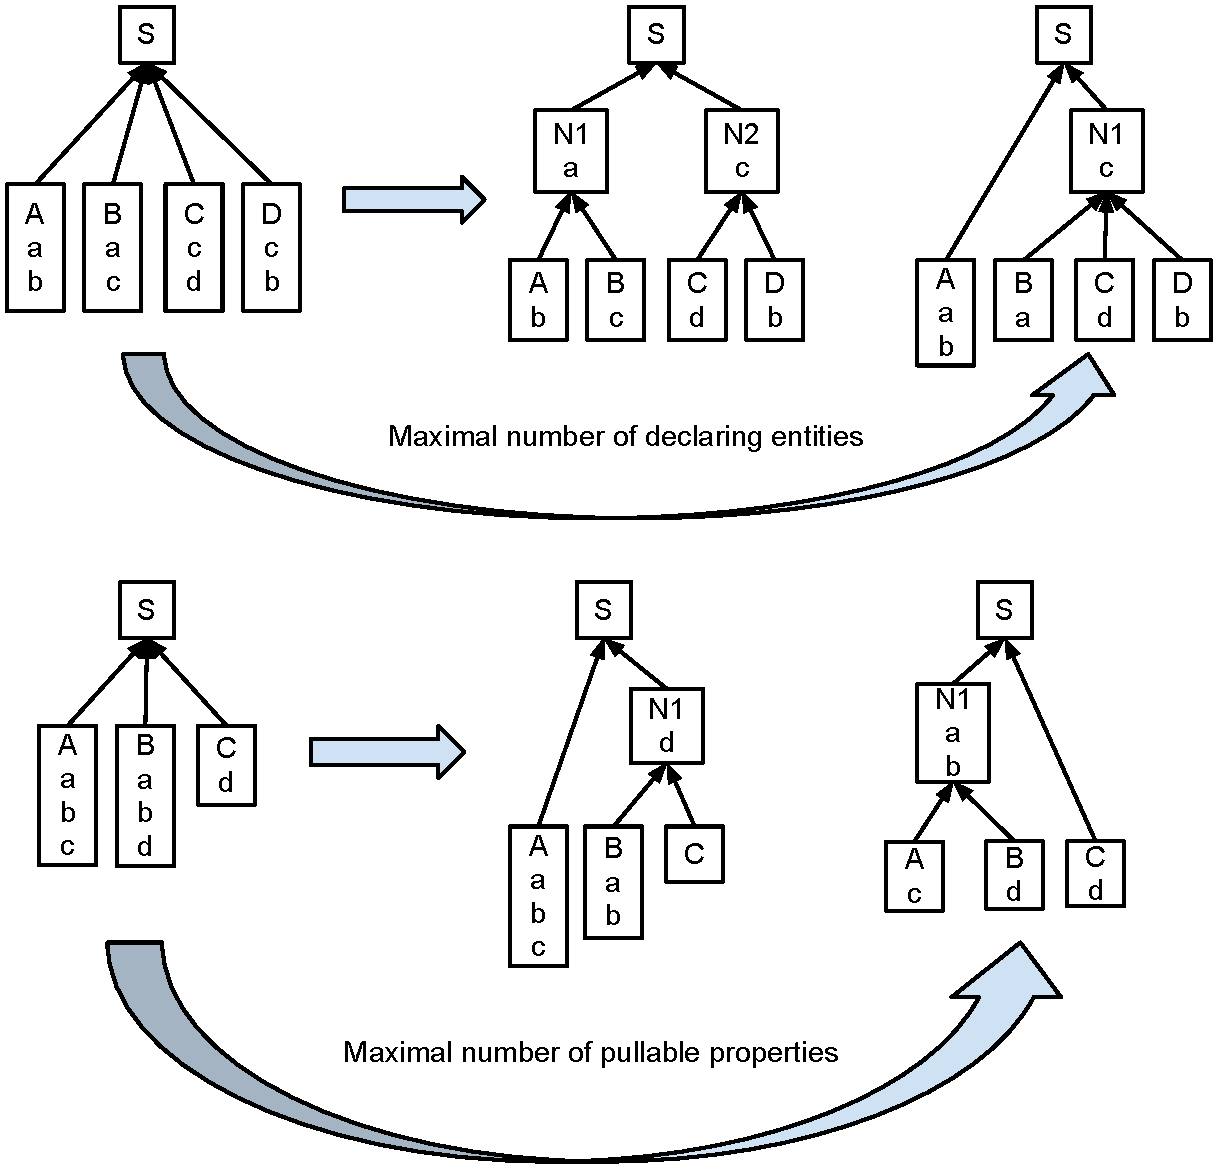
\includegraphics[width=\linewidth]{heuristics-example}
  \caption{Examples for the heuristics}
  \label{fig:heuristics-example}
\end{figure}

Figure~\ref{fig:heuristics-example} illustrates these heuristics with two
examples.  In the upper example, the property \verb|c| is shared by three
classes, whereas \verb|a| and \verb|b| are shared by only 2 classes each.  If
the transformation pulls up \verb|a| first into a new class, \verb|c| can be
pulled up only from \verb|C| and \verb|D| into another new class.  The number
of property declaration decreases from 8 to 6, \verb|b| and \verb|c| remain
duplicated once, and 2 new classes have been created.  If the transformation
uses the first heuristic, it pulls up \verb|c| first because that's common to
more classes than \verb|a| and \verb|b|.  This also results in 6 remaining
property declarations, \verb|a| and \verb|b| remain duplicated once, but only
one new class has been created.

In the lower example, the set of properties \verb|{a, b}| and \verb|{d}| are
shared by two classes both.  If the transformation decides to pull up \verb|d|,
the number of property declarations decreases from 7 to 6, \verb|a| and
\verb|b| remain duplicated once, and one new class has been created.  If the
transformation uses the second heuristic, it pulls up \verb|a| and \verb|b|,
and the number of property declarations decreases from 7 to 5, only \verb|d|
remains duplicated once, and again one new class has been created.

The \verb|common-props| function finds sets of pullable properties and sorts
them according to the heuristics.  It is by far the most complex function of
the transformation.  The function receives a set of entities via its
\verb|classes| parameter and returns the properties common to a maximal subset
of these entities.

\begin{clojurecode}
(defn common-props [classes]
  (let [pes (set (map (fn [pnt] [pnt (filter-by-properties [pnt] classes)])
                      (set (mapcat prop-type-set classes))))
        freq-map (apply hash-map
                        (mapcat (fn [[_ ents]] [ents (count (filter #(= ents (second %))
                                                                    pes))])
                                pes))
        collapse (fn collapse [aes]
                   (when-let [[pnt entities] (first aes)]
                     (let [[s r] (split-with (fn [[_ ents]] (= entities ents)) aes)]
                       (cons [(map first s) entities]
                             (lazy-seq (collapse r))))))]
    (collapse (into (sorted-set-by
                     (fn [[_ aes :as a] [_ bes :as b]]
                       (let [x (- (count bes) (count aes))]
                         (if (zero? x)
                           (let [x (- (freq-map bes) (freq-map aes))]
                             (if (zero? x) (compare a b) x))
                           x))))
                    pes))))
\end{clojurecode}

In line 2, \verb|pes| is bound to a set of tuples \verb|[pnt entity-set]|,
where \verb|pnt| is a \verb|[prop-name type]| tuple and \verb|entity-set| is
the set of all entities declaring such a property.  That is, \verb|pes| has the
following form\footnote{\textsf{\#\{...\} is a Clojure set literal.}}.

\begin{clojurecode*}{linenos=none}
#{[[pn1 t1] #{e1 e2 e3}]     [[pn4 t2] #{e2 e3 e4}]
  [[pn2 t2] #{e2 e3 e4 e5}]  [[pn3 t2] #{e1 e2 e3}]}
\end{clojurecode*}

In line 4, \verb|freq-map| is bound to a hash-map that maps to each set of
entities occuring in the items of \verb|pes| the number of occurences in there.
This map is used to implement the second heuristic.

In line 8, a local function \verb|collapse| is defined.  Before explaining
that, first lines 13 to 22 are to be explained.  What's done there is that the
entries of the set \verb|pes| are put into a sorted set.  The sorting order is
determined by the comparator function defined in lines 14 to 21.  It receives
two items of the \verb|pes| set, binds their \verb|entity-set|s to \verb|aes|
and \verb|bes|, respectively, and then performs these checks:

\begin{compactenum}
\item If \verb|bes| contains more entities than \verb|aes|, \verb|b| should be
  sorted before \verb|a|.  This implements heuristic 1.
\item Else, if the entity set \verb|bes| occurs more often in the items of
  \verb|pes|, \verb|b| should be sorted before \verb|a|.  This implements
  heuristic 2.
\item Else, the sorting order is not important and determined by Clojure's
  standard \verb|compare| function that produces a stable ordering upon all
  objects implementing \verb|Comparable|.
\end{compactenum}

As a result, the sorted set has the following structure, i.e., items with
larger entity sets are sorted before items with smaller entity sets.

\begin{clojurecode*}{linenos=none}
#{[[pn2 t2] #{e2 e3 e4 e5}]  [[pn1 t1] #{e1 e2 e3}]
  [[pn3 t2] #{e1 e2 e3}]     [[pn4 t2] #{e2 e3 e4}]}
\end{clojurecode*}

The item with \verb|pn2| is sorted before the others because it is shared by 4
entities.  In case of equally large entity sets, the number of occurences of
the entity sets determines the sorting order, e.g., the items with \verb|pn1|
and \verb|pn2| are sorted before the item with \verb|pn4|, because their entity
sets occur twice whereas the entity set of \verb|pn4| occurs only once.

Finally, this set is mangled by the local \verb|collapse| function defined in
lines 8 to 12.  It simply collapses (merges) adjacent items with equal entity
sets, thus the result of the function has the following form.

\begin{clojurecode*}{linenos=none}
([([pn2 t2])          #{e2 e3 e4 e5}]
 [([pn1 t1] [pn3 t2]) #{e1 e2 e3}]
 [([pn4 t2])          #{e2 e3 e4}]}
\end{clojurecode*}

Because the items of \verb|pn1| and \verb|pn3| have the same entity set, they
are merged into one item.


\paragraph{Restructuring Rules.}

The solution defines the function \verb|pull-up-helper| shown in
Listing~\ref{lst:pull-up-helper} which can implement all three restructuring
rules by parameterizing it appropriately.  The function receives the root
\verb|model| object \verb|mo|, a superclass \verb|super|, and a set of entities
\verb|classes| in which to find common properties,.  In case of rule 1 and rule
2, \verb|super| is the superclass of all \verb|classes|, and in case of rule 3,
the \verb|super| parameter is \verb|nil| and \verb|classes| is the set of
top-level classes.

\begin{listing}[htbp]
  \begin{clojurecode}
(defn pull-up-helper [mo super classes]
  (when (seq classes)
    (when-let [[pnts entities] (first (common-props classes))]
      (if (and super (= classes entities))
        (pull-up mo pnts entities super)  ;; rule 1
        (when (> (count entities) 1)
          (let [nc (make-entity! mo)]     ;; rule 2 if super, else rule 3
            (pull-up mo pnts entities nc)
            (doseq [s entities]
              (doseq [oldgen (eget s :generalization)
                      :when (= super (adj oldgen :general))]
                (edelete! oldgen))
              (make-generalization! mo s nc))
            (when super (make-generalization! mo nc super))
            true))))))
  \end{clojurecode}
  \caption{A restructuring function able to implement all three rules}
  \label{lst:pull-up-helper}
\end{listing}

When the set of classes is not empty (line 2), and if there are common
properties (line 3), the largest list of common properties among the lists of
properties declared by a maximal number of entities is bound to \verb|pnts|,
and the entities declaring these properties are bound to \verb|entities|.

In case \verb|entities| equals the set of all \verb|classes| (line 4), the
situation is that of rule 1, and all properties in \verb|pnts| are pulled up to
\verb|super| (line 5).

In the other case, the maximal set of common properties is shared by a maximal
but strict subset of \verb|classes|.  Here, it has to be ensured that there are
more than one entity declaring these properties (line 6), because else the
inheritance depth would increase without removing declarations.  Then, the
situation is that of rule 2 if \verb|super| is non-nil, and the situation is
that of rule 3 if \verb|super| is nil.  In any case, all shared properties are
pulled into a new entity \verb|nc|, and the generalizations are adapted.

The overall transformation function simply calls the \verb|pull-up-helper|
function shown above with appropriate parametrization as long as it can find a
match.


\paragraph{Multiple Inheritance Extension.}

The solution discussed so far works well also if the initial model already
contains multiple inheritance.  However, they won't create new classes that
specialize more than one single superclass.

To exploit the presence of multiple inheritance in order to restructure the
model resulting from the core rules so that every property is declared exactly
once, the additional rule is used.  It computes the set of duplicated
properties of all classes, and then acts according these heuristics.
\begin{compactenum}
\item If one of the entities declaring the duplicated property is a top-level
  class created by the core task rules, then the other entities become
  subclasses of this entity.  The reason for only reusing top-level entities
  created by the core task is that reusing an entity that already existed in
  the original class model will make the transformation result's type hierarchy
  incompatible with that of the original model, that is, in the original model
  B was no subclass of A, but in the result model it is.
\item Else, a new entity is created as superclass of the entities, and the
  property is pulled up.
\end{compactenum}


\section{Evaluation}
\label{sec:evaluation}

The evaluation results requested by the case description
\cite{cdrestructcasedesc} are summarized in Table~\ref{tab:evaluation}.

With 110 lines of code (core + extension task), the FunnyQT solution is
reasonably \emph{concise} given that its heuristics are more advanced than the
case description required.  Due to these heuristics, its \emph{effectiveness}
is 100\% for all provided and several additional models (such as the ones
depicted in Figure~\ref{fig:heuristics-example}).  The case description defines
the \emph{complexitiy} as the sum of operator occurences, type references, and
feature references.  The FunnyQT solution consists of 161 function calls (or
calls to special forms or macros), 4 type references, and 25 feature
references.  The \emph{development effort} has been about 8 hours for the
solution plus 2 hours for writing unit tests for it.

\begin{table}[htb]
  \footnotesize
  \centering
  \begin{tabular}{| l | l |}
    \hline
    \textbf{Measure}            & \textbf{Value}\\
    \hline
    \textbf{Size (LOC)}         & 90 (core only), 105 (core + extension)\\
    \textbf{Complexity}         & 190 = 161 funcalls + 4 type refs + 25 feature refs\\
    \textbf{Effectiveness}      & 100\%\\
    \textbf{Development effort} & approx. 8 hours (solution) + 2 hours (tests)\\
    \textbf{Execution time}     & 6 secs for the largest model (\verb|testcase2_10000.xmi|)\\
    \textbf{History of use}     & approx. 1 year\\
    \textbf{No. of case studies}& published: the 3 TTC13 cases, unpublished: approx. 20\\
    \textbf{Maximum capability} & approx. 2 million elements on SHARE\\
    \hline
  \end{tabular}
  \caption{Evaluation measures}
  \label{tab:evaluation}
\end{table}

The detailed \emph{execution times} rounded to whole milliseconds on SHARE for
all provided models are depicted in Table\ref{tab:exec-times}.  The largest
provided model consisting of 100000 elements\footnote{The models
  \textsf{testcase2\_n} actually consist of $10\times n$ elements.} can be
processed in about six seconds which is more than a thousand times faster than
the reference UML-RSDS solution.  It can be seen that the additional multiple
inheritance rule has only little influence on the execution times.

\begin{table}[htb]
  \footnotesize
  \centering
  \begin{tabular}{| l | r | r |}
    \hline
    \textbf{Model}    & \textbf{Core task only} & \textbf{Core and Extension task}\\
    \hline
    \textsf{testcase1}         & 1 ms      & 1 ms\\
    \textsf{testcase2}         & 1 ms      & 1 ms\\
    \textsf{testcase2\_1000}   & 418 ms    & 434 ms\\
    \textsf{testcase2\_5000}   & 2455 ms   & 2585 ms\\
    \textsf{testcase2\_10000}  & 5656 ms   & 6041 ms\\
    \textsf{testcase3}         & 248 ms    & 268 ms\\
    \hline
    \textsf{...}               & ...        & ...\\
    \textsf{testcase2\_200000} & 1006848 ms & 1045648 ms\\
    \hline
  \end{tabular}
  \caption{Detailed execution times on SHARE}
  \label{tab:exec-times}
\end{table}

\begin{sloppypar}
  To determine the \emph{maximum capability} of the solution, models up to two
  millions of elements have been created.  Given the limited amount of 800 MB
  memory available to the JVM process on SHARE, the model with 2 million
  elements is approximately the maximum capability for the FunnyQT solution.
\end{sloppypar}

\FloatBarrier

\bibliographystyle{alpha}
\bibliography{ttc13-funnyqt-cd-restruct}


\end{document}




%%% Local Variables:
%%% mode: latex
%%% TeX-engine: pdflatex-shell-escape
%%% TeX-master: t
%%% End:
